% Autor: Leonhard Segger, Alexander Neuwirth
% Datum: 2017-10-30
\documentclass[
	% Papierformat
	a4paper,
	% Schriftgröße (beliebige Größen mit „fontsize=Xpt“)
	12pt,
	% Schreibt die Papiergröße korrekt ins Ausgabedokument
	pagesize,
	% Sprache für z.B. Babel
	ngerman
]{scrartcl}

% Achtung: Die Reihenfolge der Pakete kann (leider) wichtig sein!
% Insbesondere sollten (so wie hier) babel, fontenc und inputenc (in dieser
% Reihenfolge) als Erstes und hyperref und cleveref (Reihenfolge auch hier
% beachten) als Letztes geladen werden!

\usepackage{tikz}
\usetikzlibrary{calc,patterns,angles,quotes} % loads some tikz extensions\usepackage{tikz}
\usetikzlibrary{babel}

% Silbentrennung etc.; Sprache wird durch Option bei \documentclass festgelegt
\usepackage{babel}
% Verwendung der Zeichentabelle T1 (Sonderzeichen etc.)
\usepackage[T1]{fontenc}
% Legt die Zeichenkodierung der Eingabedatei fest, z.B. UTF-8
\usepackage[utf8]{inputenc}
% Schriftart
\usepackage{lmodern}
% Zusätzliche Sonderzeichen
\usepackage{textcomp}

% Mathepaket (intlimits: Grenzen über/unter Integralzeichen)
\usepackage[intlimits]{amsmath}
% Ermöglicht die Nutzung von \SI{Zahl}{Einheit} u.a.
\usepackage{siunitx}
% Zum flexiblen Einbinden von Grafiken (\includegraphics)
\usepackage{graphicx}
% Abbildungen im Fließtext
\usepackage{wrapfig}
% Abbildungen nebeneinander (subfigure, subtable)
\usepackage{subcaption}
% Funktionen für Anführungszeichen
\usepackage{csquotes}
\MakeOuterQuote{"}
% Zitieren, Bibliografie
\usepackage[sorting=none]{biblatex}


% Zur Darstellung von Webadressen
\usepackage{url}
%chemische Formeln
\usepackage[version=4]{mhchem}
% siunitx: Deutsche Ausgabe, Messfehler getrennt mit ± ausgeben
\usepackage{floatrow}
\floatsetup[table]{capposition=top}
\usepackage{float}
% Verlinkt Textstellen im PDF-Dokument
\usepackage[unicode]{hyperref}
% "Schlaue" Referenzen (nach hyperref laden!)
\usepackage{cleveref}
\sisetup{
	locale=DE,
	separate-uncertainty
}
\bibliography{BA-C-04_V06_29-04-2019_References.bib}

\begin{document}

	\begin{titlepage}
		\centering
		{\scshape\LARGE Versuchsbericht zu \par}
		\vspace{1cm}
		{\scshape\huge V06 - $\beta$-Zerfall \par}
		\vspace{2.5cm}
		{\LARGE Gruppe BA-C-04 \par}
		\vspace{0.5cm}

		{\large Alexander Neuwirth (E-Mail: a\_neuw01@wwu.de) \par}
		{\large Leonhard Segger (E-Mail: l\_segg03@uni-muenster.de) \par}
		\vfill

		durchgeführt am 29.04.2019\par
		betreut von\par
		{\large Lucia Anna Husová}

		\vfill

		{\large \today\par}
	\end{titlepage}
	\tableofcontents
	\newpage


	\section{Kurzfassung}
	% Hypothese	und deren Ergebnis, wenn Hypothese ist, dass nur Theorie erfüllt, sagen: Erwartung: Theorie aus einführung (mit reflink) erfüllt
	% Ergebnisse, auch Zahlen, mindestens wenn's halbwegs Sinn ergibt
	% Was wurde gemacht
	% manche leute wollen Passiv oder "man", manche nicht
	Es wird ein Toroid-Spektrometer verwendet, um das Energiespektrum des ausgesandten Elektrons beim $\beta$-Zerfall von $^{137}$Cs zu bestimmen.
	Mit Hilfe dieses Spektrums wird durch einen Kurzie-Plot die Grenzenergie des Übergangs in den angeregten Zustand des entstehenden Ba-137 bestimmt.
	Dazu wird das Spekrtum zunächst um Elektronen anderer Quellen korrigiert.
	Die Bestimmung der Übergangsenergie ist insofern erfolgreich, als dass das Ergebnis von \SI{538 \pm 10}{keV} um weniger als \SI{10}{\percent} und um weniger als die dreifache Standardunsicherheit vom Literaturwert abweicht.
	Die Abweichung wird diskutiert und Methoden zur genaueren Bestimmung nahegelegt.
	Außerdem wird  die Impulsauflösung des Spektrometers bestimmt.

  \section{Theorie}
	% wdh. Texte
	% wdh. Besprechung
	Die untersuchte Quelle enthält $^{137}$Cs.
	Dessen Zerfallsschema ist in \cref{fig_Zerfallsschema} dargestellt.
	Man sieht, dass es jeweils über $\beta^-$-Zerfall mit einer Wahrscheinlichkeit von etwa \SI{95}{\percent} zu einem angeregten Zustand von $^{137}$Ba und ansonsten direkt in den Grundzustand zerfällt.

	\begin{figure}[H]
			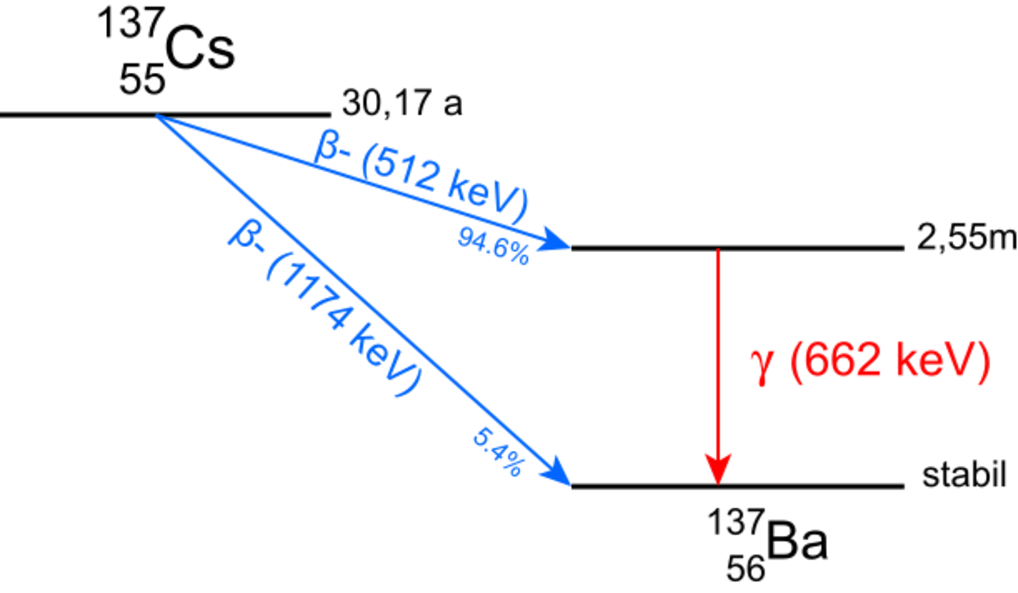
\includegraphics[width= 0.6 \linewidth]{img/cs-137-zerfallsschema}
			\caption{
			Zerfallsschema von $^{137}$Cs.
			Es gibt außer den zwei aufgeführten Endzuständen auch noch einen weniger angeregten zwischen dem Grundzustand und dem \SI{95}{\percent}-igem Endzustand.
			Dieser tritt jedoch nur mit einer vernachlässigbaren Wahrscheinlichkeit von \SI{0.0006}{\percent} auf.
			\cite{Leifi}
			}
			\label{fig_Zerfallsschema}
	\end{figure}


		Beim $\beta^-$-Zerfall findet die folgende Kernreaktion statt:
		\begin{equation}
			\label{eq_beta-minus}
			 _{55}^{137}\text{Cs} \rightarrow _{56}^{137}\text{Ba} + \text{e}^- + \bar{\nu_{\text{e}}}
		\end{equation}
		Hierfür wird im Kern ein Neutron in ein Proton, ein Elektron und ein Anitelektronneutrino umgewandelt.

		Da im Impulserhaltungssatz hier die Impulse von drei Teilchen eine Rolle spielen, nimmt das Elektron nach dem Zerfall keine diskrete Energie (wie der Heliumkern beim $\alpha$-Zerfall) an, sondern ergibt ein kontinuierliches Spektrum.

		Um trotzdem die Übergangsenergie des Zerfalls messen zu können, muss das hochenergetiche Ende des Spektrums extrapoliert werden, da hier die gesamte Übergangsenergie in Ruheenergie und kinetische Energie des Elektrons übergeht.
		Die Ruheenergie des Neutrinos muss hierbei vernachlässigt werden. %TODO confirmen
		Dies ist aber nach aktuellem Forschungsstand innerhalb der Messunsicherheiten problemlos möglich. %TODO theoretisch bräuchte man hier ne Referenz
		Mit der Übergangsenergie $E_0$ ist im Folgenden aber nur die kinetische Energie des Elektrons gemeint, sodass hier seine Ruheenergie nicht miteinbezogen werden muss.



	\section{Methoden}
	% Bilder von der Website klauen
	% einer will Präsens
	\subsection{$\beta$-Spektrometer}
	Das Halbkreisspektrometer nutzt die Tatsache, dass geladene Teilchen im magnetischen Feld eine Kreisflugbahn mit Radius in Abhängigkeit von der kinetischen Energie des Teilchens vollführen.
	Im verwendeten Spektrometer wird dabei der Radius für verschiedene Energien konstant gehalten, indem das Magnetfeld verändert wird.
	Um auch die Vaiation des Radius berücksichtigen zu können und vergleichbare Ergebnisse zu erzielen, wird häufig und auch im Folgenden die Auftragung gegen das Produkt aus Magnetfeld $B$ und Radius $\rho$ gewählt.
	Wegen der festen Detektorposition kann immer nur ein ausgewähltes Energiefenster gemessen werden.
	Hierbei tritt der Effekt auf, dass die Teilchen (hier Elektronen) in den Detektor durch den Eintrittsspalt nicht als paralleler Strahl eintreten.
	Dies führt zu Elektronen gleichem betragsmäßigen Impulses, aber unterschiedlicher Impulsrichtung, die alle das Messfenster (vgl. \cref{fig_Halbkreisspektrometer}) erreichen.
	Nach Zurücklegen eines Halbkreises ist die hieraus resultierende Strahlbreite $\Delta X$ minimal, weshalb durch diesen Aufbau eine Fokussierung in der Impulsrichtung erreicht wird, wodurch mehr Elektronen nachgewiesen werden können.

	\begin{figure}[H]
			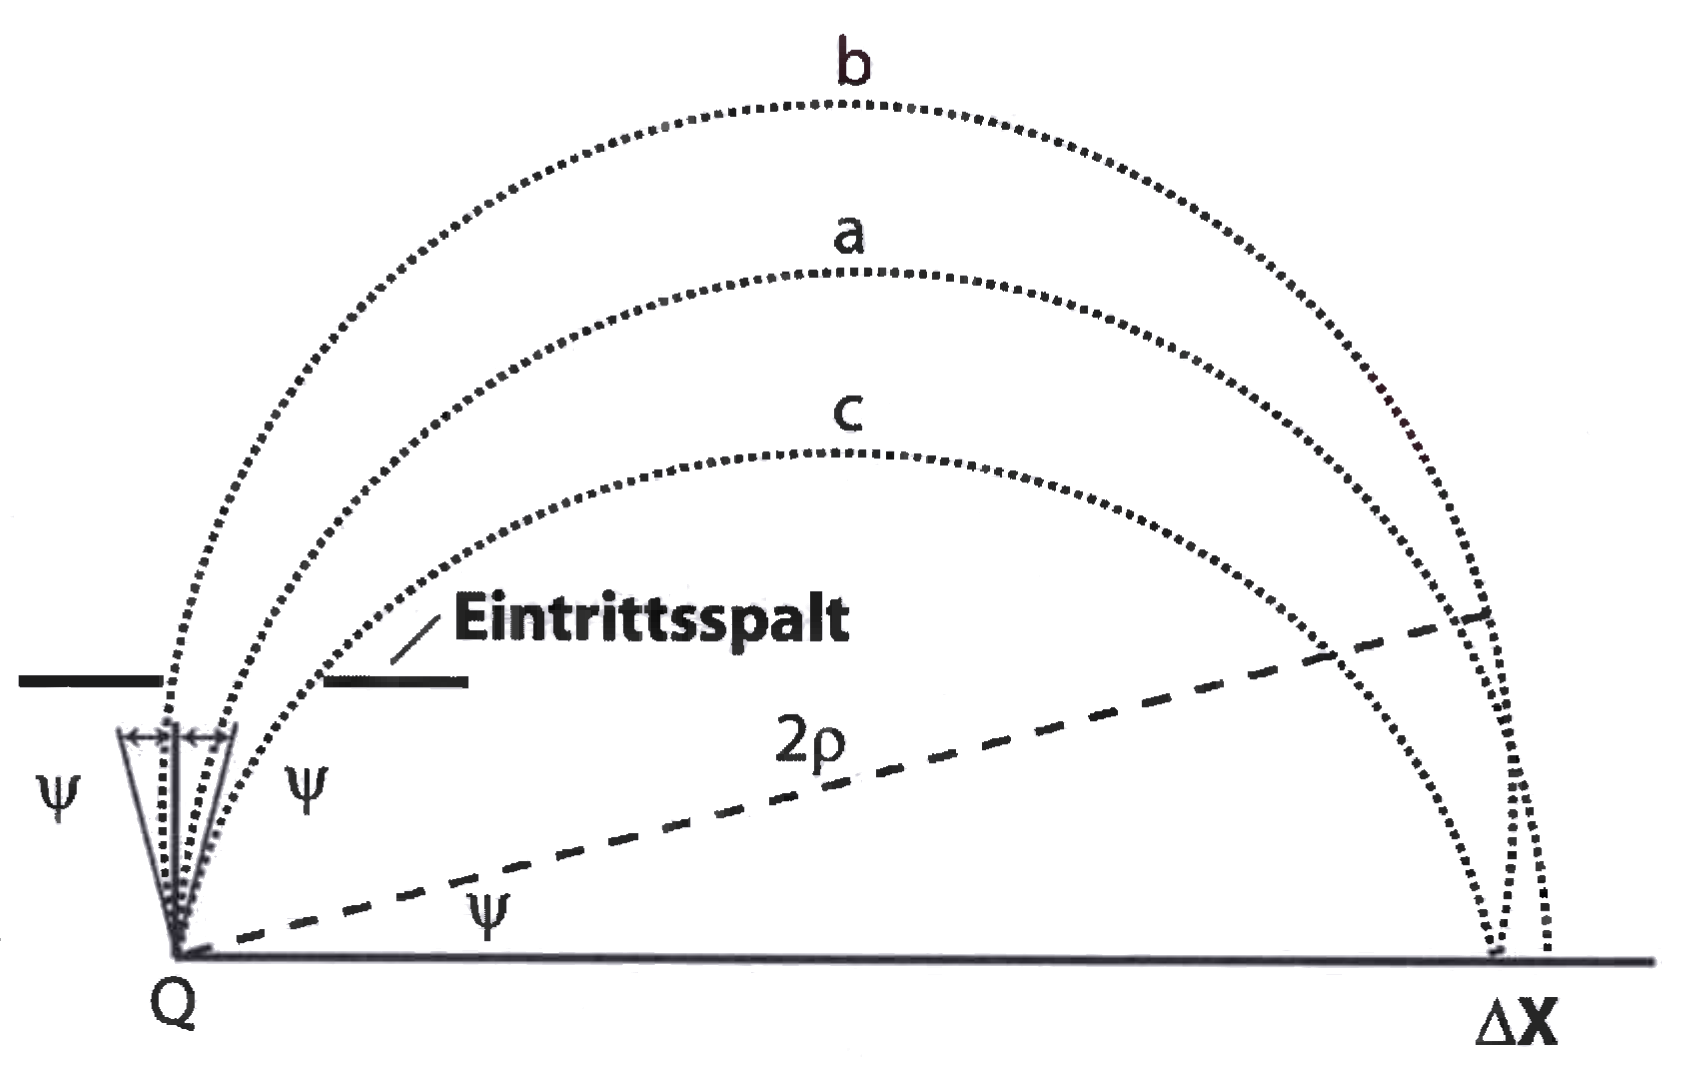
\includegraphics[width= 0.6 \linewidth]{img/spektrometer_schema}
			\caption{
			Fokussierungsprinzip eines Halbkreisspektrometers.
			\cite{Anleitung}
			}
			\label{fig_Halbkreisspektrometer}
	\end{figure}

	Eine zusätzliche Fokussierung kann erreicht werden, indem ein radialsymmetrisches Feld verwendet wird, welches mit $1/4$ abnimmt.
	Dies sorgt für eine Fokussierung in beide Streurichtungen der eintretenden Elektronen.
	Der Detektor ist dementsprechend keilförmig geformt. %TODO muss zugeben, das Kapitel in der Anleitung nicht recht verstanden zu haben...

	Für die Erzeugung des Magnetfelds wird ein Spule verwendet.
	Hier ist aufgrund der Restmagnetisierung des Materials eine Hysteresekurve anstelle eines gleichmäßigen linearen Zusammenhangs zwischen Strom und Magnetfeld zu erwarten.
	Gemäß \cite{Anleitung} kann der Zusammenhang innerhalb des Messbereiches jedoch als linear angenommen werden.
	Es wird aber immer bei hohen Spannungen angefangen zu messen, da dann immer der gleiche Hysteresepfad gewählt wird.

	Die Elektronen werden mit einem Szintillator in Verbindung mit einem Photomultiplier detektiert.
	Das Signal wird nach dem Vorverstärker in den Hauptverstärker geleitet und dann über den gewählten Messzeitraum akkumuliert und digitalisiert.

	\subsection{Messung des Spektrums}

	Für die Messung wird das Spektrometer mit einer Vakuumpumpe evakuiert.
	Zunächst wird das Spektrum in Schritten von \SI{1}{V} \SI{60}{\minute} lang gemessen.
	Mithilfe dieser Messung wird dann das Spektrum in mehrere Teile eingeteilt.
	Dabei werden den Bereichen, in denen vorallem der Untergrund gemessen wird, lange Messdauern und hohe Schrittweiten zugewiesen, während in Bereichen hoher Messrate kurze Messzeiträume und geringe Schrittweiten verwendet werden.
	Dies erlaubt, dass nahe der Peaks besonders kleinschrittig gemessen wird, während in den Bereichen geringer Ereignisrate noch immer ausreichend Ereignisse gemessen werden.
	Mit dieser Einteilung wird das Spektrum dann über einen Zeitraum von \SI{6,5}{\day} gemessen.
	Zur Aufnahme und Speicherung sowie Steuerung der Messparameter wird ein LabVIEW-Programm geschrieben und verwendet.

	\begin{figure}[H]
			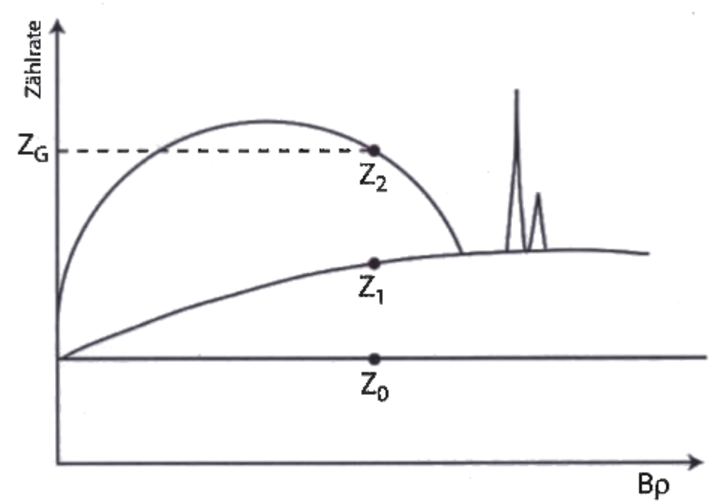
\includegraphics[width= 0.6 \linewidth]{img/Schema_Spektrum}
			\caption{
			Schematisches erwartetes Gesamtspektrum.
			\cite{Anleitung}
			}
			\label{fig_Schema_Spektrum}
	\end{figure}

	In \cref{fig_Schema_Spektrum} ist das erwartete Spektrum in schematischer Form dargestellt.
	Z$_0$ entspricht dabei einem horizontalen Untergrund aus Hintergrundstrahlung.
	Z$_1$ ist der oben erwähnte Zerfall in den Grundzustand von $^{137}$Ba, der später als näherungsweise linear angenommen wird.
	Z$_2$ stellt den gesuchten Zerfall in den angeregten Zustand dar.
	Die beiden schmalen Peaks treten durch Konversionselektronen von K- und L-Schale auf.
	Sie sollen im Folgenden zur Kalibrierung des Spektrums verwendet werden.

	Konversionselektronen treten dadurch auf, dass, wenn das angeregte $^{137}$Ba in den Grundzustand übergeht und der Energieübertrag zur Aussendung eines Elektrons aus der K- oder L-Schale führt.

	\section{Ergebnisse und Diskussion}


	\subsection{Beobachtung und Datenanalyse}
	% Allgemeine Beobachtungen
	% Einflüsse von veränderten Parametern auf Messung
	%\subsubsection{Unsicherheiten}
	% Berechung nach Aufgabenstellung
	\subsubsection{Unsicherheiten}
	Alle Unsicherhieten werden nach GUM bestimmt und berechnet.
	Für diese Berechnungen wurde die Python Bibliothek \enquote{uncertainties} herangezogen, welche den Richtlinien des GUM folgt.
	Die Fits verwenden die Methode der kleinsten Quadrate.
	\subsubsection{Untergrund}
	In \cref{fg_untergrund} sind die gemessenen Ereignisraten gegen die angelegte Spannungen aufgetragen.
	Die blaue Horizontale ist jeweils an einen Bereich von \SI{0.25}{V} am Anfang und Ende der Messkurve angepasst und beschreibt so die Untergrundrate.
	Die Unsicherheit der gemessenen Ereignisse ist durch $\sqrt{N}$ gemäß Poisson-Verteilung gegeben.
	Damit folgt für die Unsicherheit der Ereignisrate $u(R)=\sqrt{N}/T$, wobei $T$ die Messdauer bei gegebener Spannung ist.
	\begin{figure}[H]
			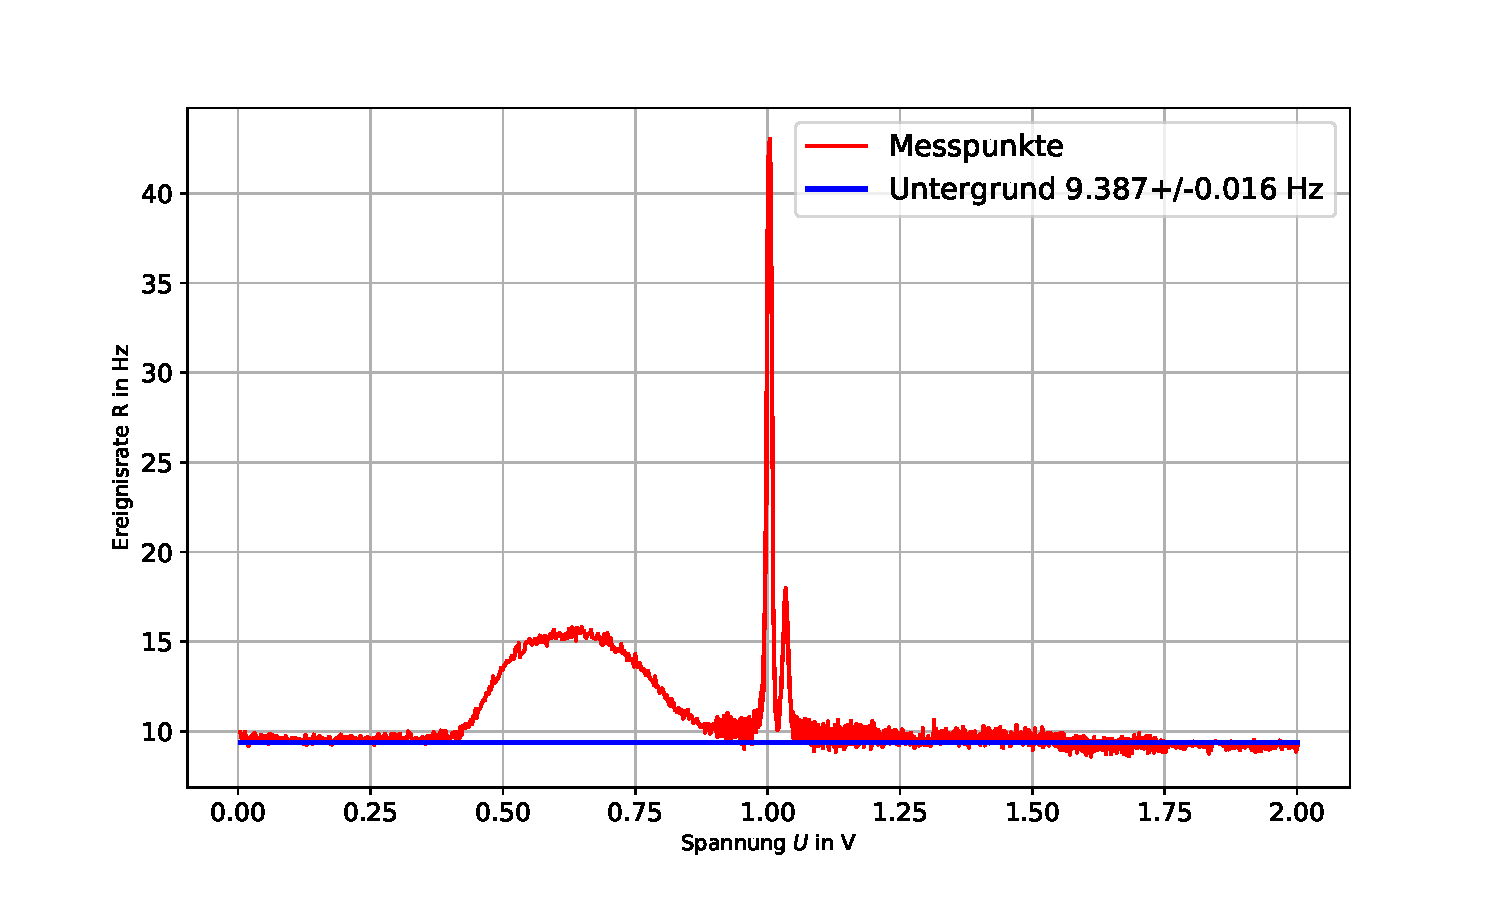
\includegraphics[width=  \linewidth]{img/untergrund}
			\caption{
			Die Anzahl der Ereignisse wurde durch die Messzeit bei einer festen Spannung dividiert, sodass sich die Ereignisrate ergibt.
			Die Unsicherheiten sind kleiner als die Symbole.
			}
			\label{fg_untergrund}
	\end{figure}

	\subsubsection{Kalibration des Spektrometers}
	Um das Spektrometer zu kalibrieren, nutzt man, dass die Konversionselektronen des $^{137}$Ba eine scharfe Energie haben.
	Diese Energien sind bekannt und in \cref{tb_konversion} aufgelistet.
	Dabei ist der Wert für die L-Linie der nach den Intensitäten der drei L-Linien gewichtete Mittelwert.

\begin{table}[H]
		\centering
		\begin{tabular}{c | c | c  }
			 Schale&E in \si{keV} & $B\rho$ in \si{Tcm} \\ \hline
			 K & \SI{624.21}{} & \SI{0.33814(5)}{} \\
			 L & \SI{655.8}{} & \SI{0.3499(1)}{} \\
		\end{tabular}
		\caption{
		Gemittelte Energie der L und K Konversionselektronen von $^{137}$Ba und zugehöriger B$\rho$-Wert. \cite{Anleitung}
		}
		\label{tb_konversion}
\end{table}
In \cref{fg_kalibration} sind die zwei Peaks vergrößert dargestellt und es wurden jeweils die Spitzen mit einer Gaußfunktion angepasst.
Außerdem wurde der zuvor bestimmte Untergrund subtrahiert.
	\begin{figure}[H]
			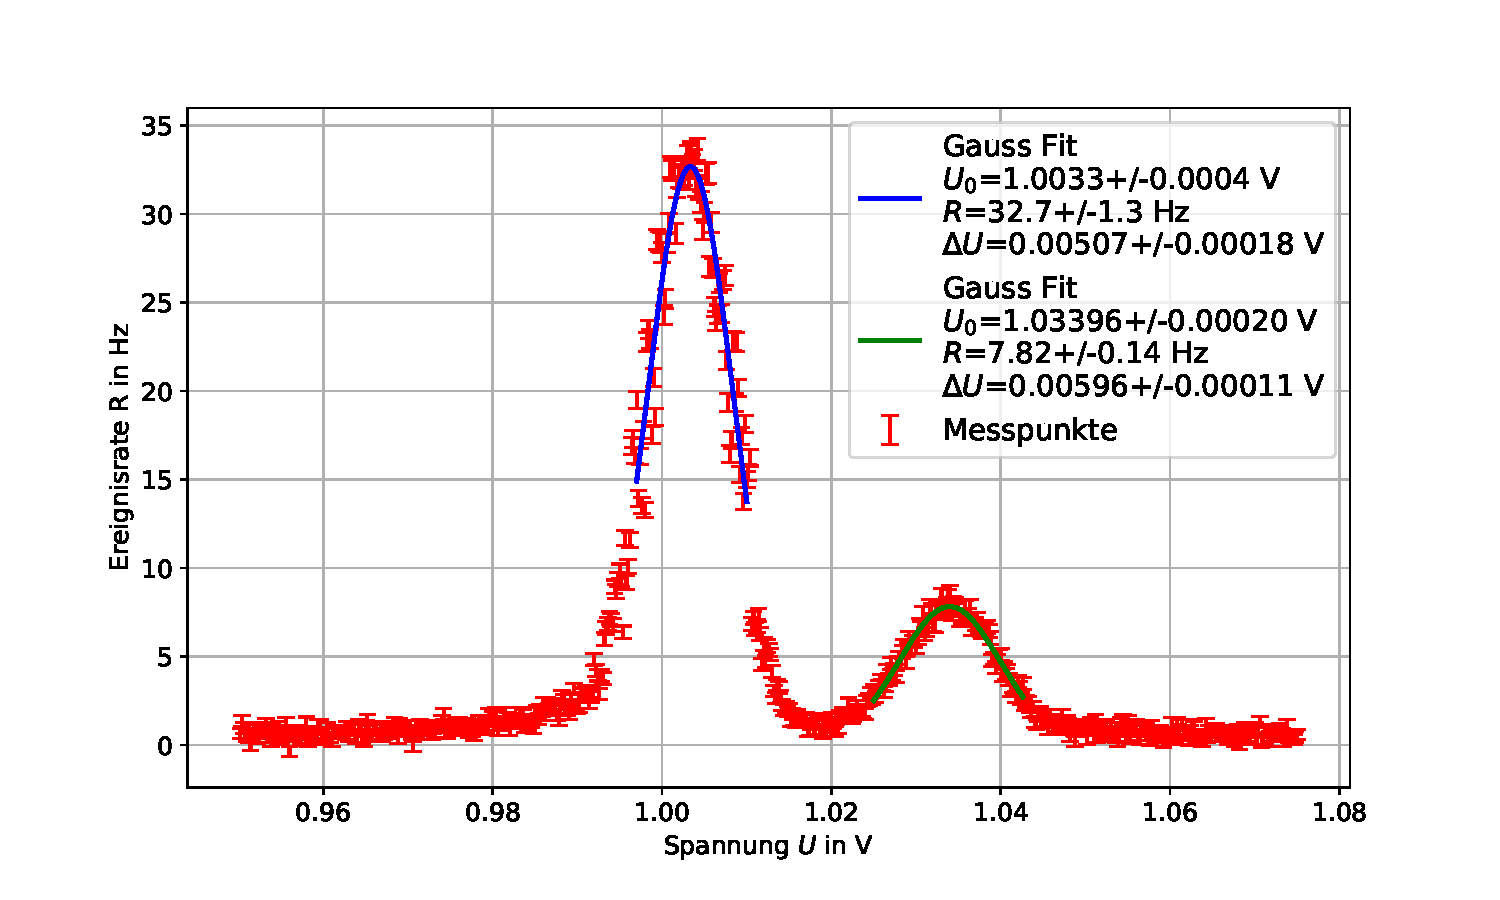
\includegraphics[width=  \linewidth]{img/kalibration}
			\caption{
			Vergrößerte und um den Untergrund reduzierte Messung der Peaks.
			Der größere Peak ist der K-Peak.
			}
			\label{fg_kalibration}
	\end{figure}

	Da mit einem Magnetspektrometer jedoch ein Impuls $p=eB\rho$ anstelle einer Energie gemessen wird, kalibriert man zunächst nach $B\rho$.
	Der Kalibrationsparameter ergibt sich aus dem Verhältnis von der Differenz der $B\rho$-Werte und dem Abstand der Peaks.
	\begin{equation}
		a = \frac{\Delta B\rho}{\Delta U_{KL}} = \frac{\SI{0.0118+-0.0001}{Tcm}}{\SI{0.031+-0.007}{V}} = \SI{0.384+-0.089}{Tcm/V}
	\end{equation}
	Für die Unsicherheit der Peakpositionen wurde die Breite des Gaußfits verwendet.
	Die gemäß \cref{eq_rho} kalibrierte Messkurve ist in \cref{fg_kali} enthalten.
	\begin{equation}
		\label{eq_rho}
		B\rho = aU-aU_{0,K}+(B\rho)_K
	\end{equation}
		Für die Impulsauflösung folgt:
	\begin{equation}
		R = \frac{\Delta B \rho}{B\rho} = \frac{2\sqrt{2\ln2}a\Delta U}{aU-aU_{0,K}+(B\rho)_K}
	\end{equation}
	Der Faktor $2\sqrt{2\ln2}$ kommt daher, dass $\Delta U$ die Standardabweichung der Gaußkurve ist, während die Definition der Impulsauflösung aber $\Delta B\rho$ als Halbwertsbreite verlangt.
	Für die zwei Peaks ergibt sich:
	\begin{align}
	R_K&= \SI{1.4+- 0.3}{\percent} \\
	R_L&= \SI{1.6+-0.4}{\percent}
	\end{align}

	\label{sec_Aufloesung}

	\subsubsection{Kurie-Plot}

	In \cref{fg_kali} wird der Beitrag durch den $\beta$-Zerfall direkt in den Grundzustand linear approximiert.
	Als Anfangspunkt für diesen wurden einige Messpunkte vor dem deutlichen Anstieg des $\beta$-Spektrums und einige unmittelbar vor dem Anstieg des L-Konversionspeaks gewählt (Siehe Anfang und Ende der blauen Linie).
	Die genaue Wahl des zweiten Punktes ist nicht wichtig, da eine Verschiebung um $\pm\SI{0.05}{Tcm}$, den Fit kaum verändert.
	Wenn man die Messkurve dann um diesen Beitrag reduziert erhält man die Ereignisrate $N(eB\rho)=N(p)$.
\begin{figure}[H]
			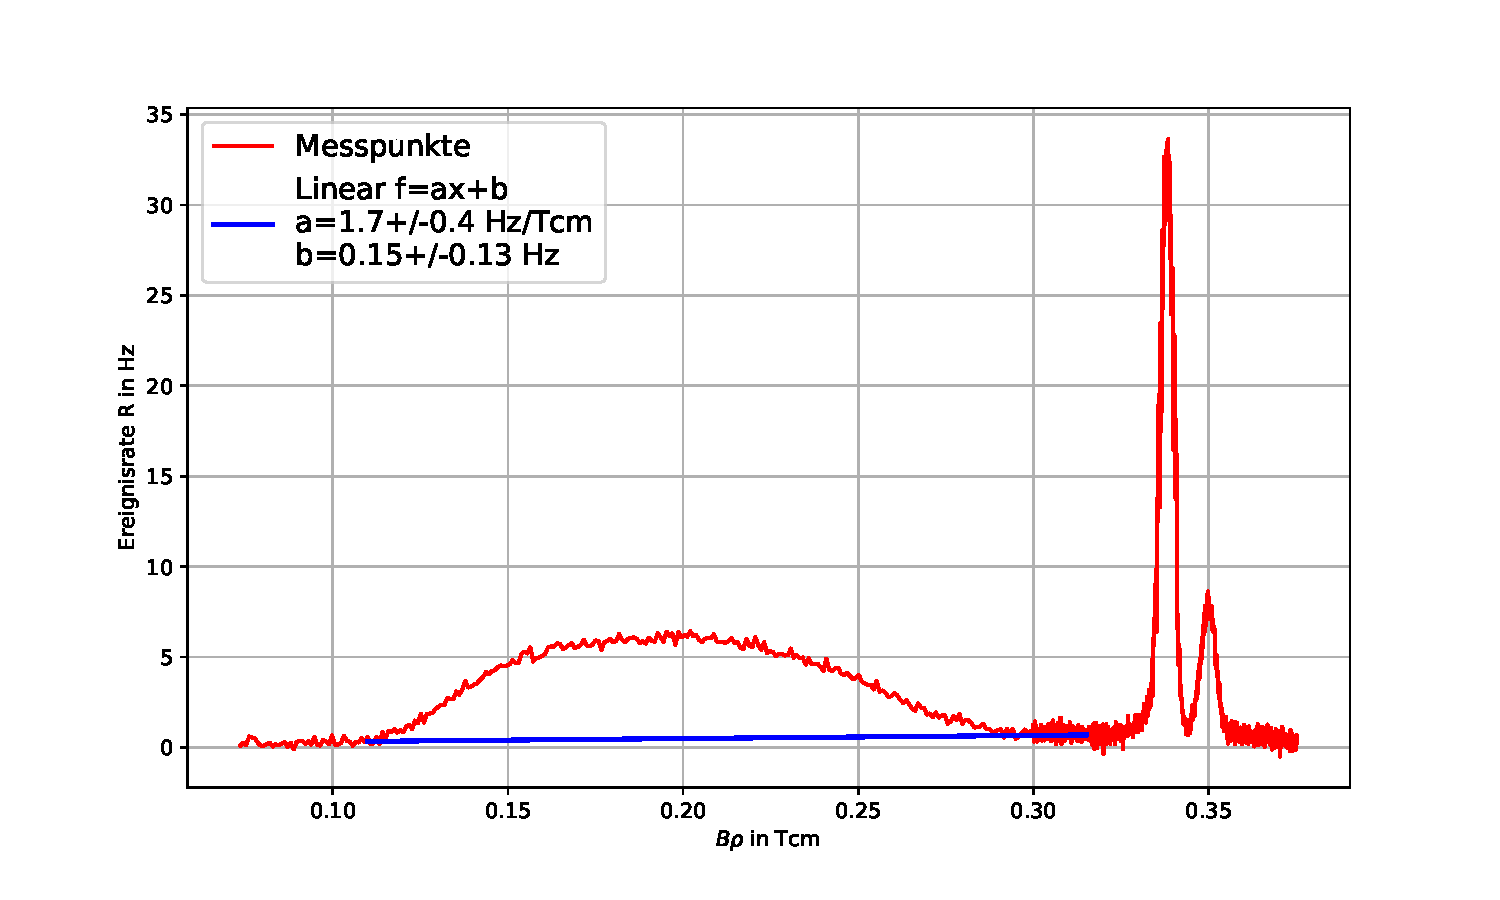
\includegraphics[width=  \linewidth]{img/kali}
			\caption{
			Um den Beitrag des direkten Zerfalls in den Grundzustand und die Ränder reduzierte kalibrierte Messung.
			Die Unsicherheiten sind kleiner als die Symbole.
			}
			\label{fg_kali}
	\end{figure}
	$N(p)$ lässt sich zum Kurie-Plot gemäß
	\begin{equation}
		K(p) = \sqrt{\frac{N(p)}{F(Z,E)p^2}}
	\end{equation}
	mit
	\begin{equation}
		F = \frac{k}{1-\exp^{-k}} \quad \textrm{und} \quad k=\frac{2\pi Z \alpha c}{v}
	\end{equation}
	transformieren.
	$F$ ist die genäherte Fermifunktion und ist notwendig für die Coulombkorrektur durch die Kernladung $Z$.
	$\alpha$ ist die Feinstrukturkonstante.
	Relativistisch gilt für die Geschwindigkeit $v$ des Elektrons.
	\begin{equation}
		v = \frac{p}{\gamma m} = \frac{p\sqrt{1-(v/c)^2}}{m}
	\end{equation}
	Nun quadriert man und formt nach $v^2$ um:
	\begin{equation}
		v^2 = \frac{p^2}{m^2c^2} (c^2-v^2) = \frac{p^2}{m^2} \frac{1}{1+p^2/(mc)^2} = \frac{p^2}{m^2+(p/c)^2}
	\end{equation}

	Für die Kurie-Darstellung gilt $K(p)\propto (E_0-E)$ \cite{Anleitung}.
	Damit erhält man die Energie des $\beta$-Zerfalls als Schnittpunkt mit der x-Achse, wenn man die x-Achse von $B\rho=p/e$ zu $E_{kin}=\sqrt{p^2c^2+m^2c^4}-mc^2$ umskaliert.
	Das Ergebnis dieser Umformungen ist in \cref{fg_kurie} abgebildet.
	\begin{figure}[H]
			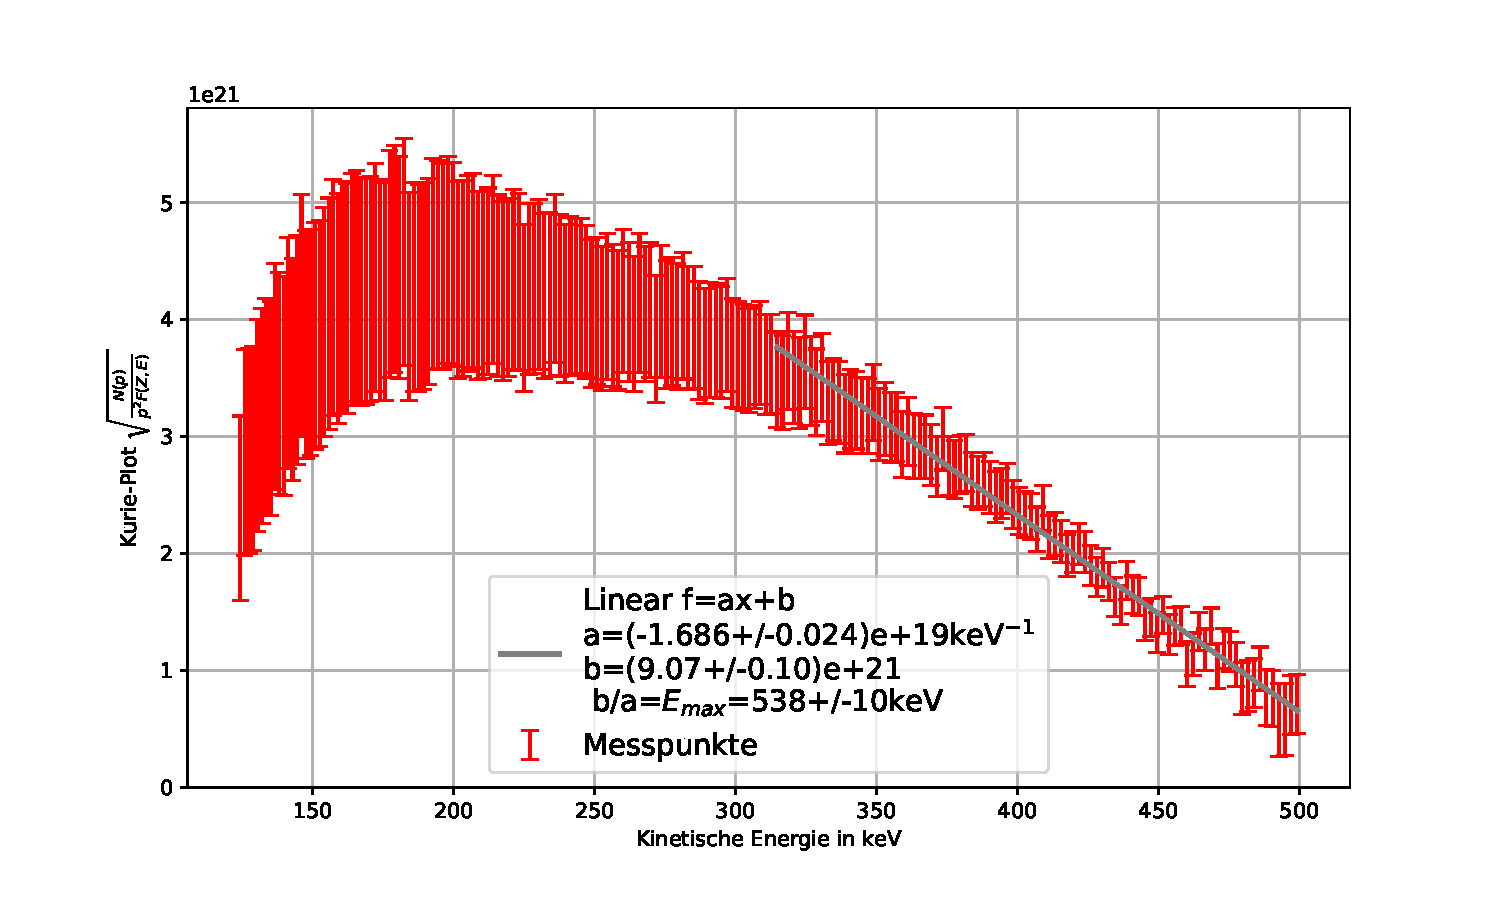
\includegraphics[width=  \linewidth]{img/kurie}
			\caption{
			Kurie-Darstellung der Messung.
			}
			\label{fg_kurie}
	\end{figure}
	Als maximale kinetische Energie des Elektrons, die der $\beta$-Zerfallsenergie entspricht, ergibt sich $E_0=E_{max}=\SI{538+-10}{keV}$.
	\subsection{Diskussion}
	% Bezug/Nutzen oder sonst was
	% auch hier die Hypothese wiederholen
	% keine Messwerte hier, nach manchen Menschen, zumindest "direkt" erstellte Diagramme net hier, auch wenn Lesbarkeit-bla
	Zunächst lässt sich sagen, dass das gemessene Spektrum (vgl. \cref{fg_untergrund}) prinzipiell dem schematisch erwarteten Spektrum (vgl. \cref{fig_Schema_Spektrum}) entspricht.
	Da der Zerfall in den Grundzustand nur mit einer Wahrscheinlichkeit von etwa \SI{5}{\percent} auftritt, ist es nicht überraschend, dass er im Spektrum am schwersten zu erkennen ist.
	Das Kalibrieren anhand der Peaks ist möglich, da diese eindeutig zu identifizieren sind.

	Bei der Betrachtung von \cref{fg_kurie} fällt zunächst auf, dass der erwartete lineare Zusammenhang in der Kurie-Darstellung für hohe Energien erkennbar ist, aber für geringere Energien stark anders aussieht.
	Dies wird einerseits darauf zurückgeführt, dass die Kalibrierung weit vom Kalibrierpunkt entfernt weniger präzise wird, was ein Grund für die Abweichung sein kann.
	Andererseits ist zu erwähnen, dass das Abziehen des Einflusses des Übergangs in den Grundzustand durch einen linearen Fit zu Abweichungen führen kann, da es sich lediglich um eine Approximation erster Ordnung des eigentlichen Verlaufs handelt.
	Bei Betrachtung von \cref{fig_Schema_Spektrum} sieht man, dass die Linearität vorallem für höhere Energien gegeben ist, was die Vermutung, dass dies ein Grund für die Abweichungen ist, bekräftigt.

	Außerdem führt die Fehlerfortpflanzung zu einem größeren Fehler bei kleiner Energie, wie ebenfalls aus \cref{fg_kurie} entnommen werden kann.
	Dies drückt sich auch in der Impulsauflösung aus, die wie es in \cref{sec_Aufloesung} beim Peak, anhand dessen kalibriert wurde, auftritt, besser ist als an dem anderen Peak.
	Dies lässt sich für das gesamte Spektrum annehmen.
	Sie liegt wie nach \cite{Anleitung} üblich in der Nähe von \SI{1}{\percent}.

	Die bestimmte Übergangsenergie $E_0=\SI{538+-10}{keV}$ ist nun mit dem Literaturwert von \SI{512}{keV} gemäß \cite{Leifi} zuvergleichen.
	Der Literaturwert liegt innerhalb der dreifachen Unsicherheit des Messwerts und die Abweichung ist geringer als \SI{10}{\percent}.
	Diese Abweichung ist ebenfalls auf die oben genannten Gründe zurückzuführen.



	% lineare approx ist am hohen Ende nicht mehr so gut
	\section{Schlussfolgerung}
	% Rückgriff auf Hypothese und drittes Nennen dieser
	Insgesamt gesehen lässt sich sagen, dass die Messung der Zerfallsenergie von $^{137}$Cs erfolgreich war.
	Der Messwert weicht ausreichend gering vom Literaturwert ab, als dass dieser als bestätigt angesehen werden kann.
	Um die Abweichung zu reduzieren, könnte ein passenderer Fit für den Abzug des Übergangs in den Grundzustand gewählt werden.
	Auch die Kalibrierung könnte präziser durchgeführt werden, indem einzelne Messungen mit Proben mit bekannten Konversionspeaks durchgeführt werden würden.
	Hierfür könnten Proben mit Peaks im Bereich geringerer Energien ausgewählt werden, wodurch die Abweichung durch Messpunkte weit entfernt von den Kalibrierpunkten ausgeschlossen werden.

	% Quellen zitieren, Websiten mit Zugriffsdatum
	% Verweise auf das Laborbuch (sind erlaubt)
	% Tabelle + Bilder mit Beschriftung
	\printbibliography
\end{document}
